\section{Introduction}
In the previous chapter we saw theories of how mountain differ from plains structurally. In this chapter we will study the Duvergers law in the Indian context and analyse its implications on the mountain and plain polities.  We will look at the dataset, methodology and trends along with a brief explanation of the trends. This chapter aims to uncover whether the political structures of India's mountain states differ systematically from those of the Indo-Gangetic plains, and how these differences manifest within the electoral process.  We complement the analysis of Duverger's law with a high level social study using parameters from the National Family Health Survey (NFHS). We will explore why the parameters were chosen and what they show to us and then compare results for mountains and plains.
\section{Duvergers Law}
Maurice Duverger, a prominent French political scientist introduced a principle in the mid-20th century that has since become foundational in the study of electoral systems. Duverger's law states that electoral systems that follow a single-member plurality system (SMPS) such as India where the winner takes all tend to result in the dominance of two major political parties. Popular examples for this are the USA and UK elections, where this has been observed. However, this is not a firm law as it does not hold in India and Canada.
Two primary mechanisms have been identified through which electoral systems influence party structures in relation to Duvergers law:
 \begin{enumerate}
     \item \textbf{Mechanical effect:}  In a single member plurality system, the party receiving the most votes wins. This means that the smaller parties often struggle to secure representation. This process causes over representation of larger parties and under representation of smaller parties leading to a concentration of political competition between two dominant parties. Often, Duverger's law has been used to study national level competitions but the essence of this law has been often identified on district level \citep{cox1997making,GALLAGHER199133,lijphart1994,rae1971political}. Increase in competition between multiple parties at a district level indicates a higher competition at national level too.
     \item \textbf{Psychological effect:} This is a direct response to the mechanical effect by the voters and political elites. For example, knowing that smaller parties have little chance of winning, voters avoid wasting their votes on them, instead opting for one of the major contenders. Similarly, political elites may choose not to enter the race under unfavorable conditions or may form coalitions to enhance their viability.
 \end{enumerate}
 The distinction between mechanical effect and psychological effect might seem blurred at first but it is important to note that there can be various reasons for voters responding to the mechanical effect. Mechanical factor can be measured using various magnitudes like the Laakso and Taagpara index \citep{laakso1979effective} or the Golosov index \citep{golosov2010effective} but it is often difficult to quantify the psychological effect. The psychological effect is not limited solely to the example mentioned above and there can be various reasons for the mechanical effect, which can often be difficult to measure. For example information flow may influence this dominance and more than two parties may emerge in single member plurality systems even when all voters are strategic \citep{clough2007strategic}. Hence, it is important to note that 

\vspace{0.3cm}

Strategic voting can be often used to explain the results of Duverger's law. It has been useful in explaining the psychological reasons behind the rise of Duverger's law. A party can manage to garner a lot of support from its constituency and still lose by a minor margin. Votes for minor parties can potentially be regarded as splitting votes away from the major parties. To counteract this, voters often engage in \enquote{strategic voting}  which occurs when voters make choices based on electoral expectations rather than sincere preferences \citep{Bol2019StrategicVV}. This behavior can take various forms, such as deserting small parties for larger ones or vice versa, depending on the electoral system. More on this will be covered later, keeping the Indian context in mind. 
 
\section{The Indian Case}
The Congress party system \citep{kothari1967india, candland1997congress} was a massive umbrella organisation observed in 1950s and 1960s as Congress originally founded to fight for reforms under British rule, the Congress evolved into a mass organization that led India to independence. It became a massive umbrella organisation to accommodate different groups that in some cases conflicted with each other and hence became a system of checks and balances allowing them to maintain a median position in India. Thus, a two party system was observed and Duverger's law was being followed \citep{riker1982two}. Since the 1970s, India's political landscape has seen the emergence of identity-based parties and increasing party fragmentation among congress as Congress started to lose its hegemony. The INC  split in 1969, resulting in the Congress (O) and Congress (R). The latter, led by Indira Gandhi, adopted more populist policies including the nationalization of banks and the abolition of privy purses. \citep{Guha2011article}. These measures aimed to address economic disparities but also led to centralization of power within the party. The traditional umbrella party structure found it challenging to maintain its dominance as deepening of these social divisions. Concurrently, identity-based political movements gained momentum\citep{farooqui2016can}. The rise of the Dalit Panthers in Maharashtra during the early 1970s exemplified this trend. Inspired by the Black Panther movement in the United States, the Dalit Panthers sought to combat caste-based discrimination and were instrumental in bringing Dalit issues to the forefront of regional politics. The 1970s also concluded the formation of North Eastern states in India. States such as Meghalaya, Manipur, and Tripura were granted statehood in 1972, followed by Arunachal Pradesh and Mizoram in 1987.  Nevertheless, these states participated in the lok sabha elections post 1975.

\vspace{0.3cm}


Following on these studies, this study will use both lok sabha and assembly level constituencies to perform its analysis. This will give us a true essence of Duvergers law and more will be elaborated in the following sections.

\section{Dataset}

The Indo-Gangetic plains serve as a relevant comparative base for analysis as many mountain states were carved out of the plains regions through various reorganization processes. A notable example is Himachal Pradesh which underwent reorganisation in 1966 following the recommendations of the States Reorganisation Commission. The contemporary political geography of the Northeast was finalized in 1975 with Sikkim's incorporation into India. The data for the analysis is compiled from the Election commission of India and the timeframe is set from 1977 to 2014. The year 1977 is chosen because almost all mountain states (except Uttarakhand) were formed by then. 

\vspace{0.3cm} 

The Indo-Gangetic Plains encompass several states and territories: Punjab, Haryana, Rajasthan, Delhi, Chandigarh, Uttar Pradesh, Bihar , West Bengal, and Assam (not a part of indo gangetic plains but part of Brahmaputra plains). For this study,  Jharkhand's share of seats have also been counted as a part of Bihar. For Northern mountains we include the states of Arunachal Pradesh, Himachal Pradesh, Manipur, Meghalaya, Mizoram, Nagaland, Sikkim, Tripura, and Uttarakhand. This analysis deliberately excludes Jammu and Kashmir due to its complex geopolitical situation and the presence of international actors has created unique political dynamics that would confound the geographic comparison being studied. Also owing to its special status, lack of complete data and political debate around it due to the now scrapped Article 370 which was active during our period of study. Article 370 gave the state a separate constitution, a state flag, and autonomy of internal administration which was unlike any other state and hence clubbing it with the rest of the mountain states would be unfavourable. We also identified the constituencies in the state of Uttarakhand before it separated from Uttar Pradesh in 2000 and incorporated them to analyse the behavior of uttarakhand before the formation of the state and removed the same constituencies from Uttar Pradesh which are Almora, Garhwal, Hardwar, Nainital, Tehri Garhwal. For assembly elections the constituencies are: Uttar Kashi, Badri Kedar, Naini Tal, Laksar, Mussoorie, Khatima, Chakrata, Roorkee, Didihat, Bageshwar, Pithoragarh, Dehradun, Lansdowne, Devprayag, Haldwani, Ranikhet, Almora, Hardwar, Pauri, Karanprayag, Kashipur, Tehri.

\vspace{0.3cm}

Assembly-level constituency data is also sourced from the Election Commission of India. Unlike Lok Sabha elections, which take place simultaneously across all states, assembly elections follow separate cycles for each state. This makes it challenging to aggregate and analyze them in the same way. To address this, we group assembly elections within a five-year window and align them to the nearest benchmark year—1975, 1980, 1985, 1990, 1995, 2000, 2005, and 2010. This allows us to identify overall trends more effectively.

\vspace{0.3 cm}

The differences between mountainous and plain regions  are rooted in fundamental structural distinctions that shape the society \citep{jamesscott}. To better understand these variations we study social indicators related to the gender dynamics. For this analysis, we use data from the National Family Health Survey (NFHS) which is a  nationwide survey that has had five major iterations—in 1992, 1998, 2005, 2015, and 2019. The NFHS consists of two primary datasets: 

\begin{itemize}
    \item The \textbf{household dataset} provides insights into household composition, living conditions, access to basic amenities, asset ownership, and broad health indicators for all household members.
\item The \textbf{individual dataset} offers more granular demographic, health, and lifestyle data. In the 1992 and 1998 iterations, this dataset focused exclusively on married women aged 15–49. From 2005 onward, the scope expanded to include women (15–49 years), men (15–54 years), and children under five.
\end{itemize}

In our analysis, we primarily examine the individual dataset of women to assess the extent of freedom across different regions. This evaluation is based on various parameters, which will be detailed further in the methodology section.

\vspace{0.3 cm}

To analyze women's literacy at the state level, data from \cite{census1991,census2001,census2011} has been utilized, along with literacy data from the \cite{NSC2017}.

\section{Methodology}
\subsection{Duverger's law}
To operationalize duverger's law, we can count the total number of parties participating in the constituency. However, this can produce false results as we need to find the major parties and the votes received by each party should be given some weight in the analysis. Instead, we use Laakso and Taagepera Index \citep{laakso1979effective} to calculate the effective number of parties in a constituency. The formula is
\begin{equation*}
N = \frac{1}{\sum_{i=1}^{n} p_i^2}
\end{equation*}
where N is the total number of political parties and $p_i$ is the proportion of votes obtained by party $i$, $p_i$ is calculated separately for each party within each constituency and weighs party by their relative strength, ensuring larger parties are given more weight than the smaller. In assessing the presence of a two-party system, the ideal value of ENP should be 2 which shows that there are two major parties in the constituency. Since the number can be non integer as well, this study employs an ENP threshold of 2.5 which has been used in various methodological frameworks established by Laakso and Taagepera, Diwakar, and Chhibber. Additionally a softer threshold of 3.0 is considered as a soft cutoff for analysis which has also been used in the above frameworks. This analysis employs both ENP thresholds to evaluate district level party competition, with the state level ENP calculated as the mean of district level values, following Diwakar's methodological approach. For each state the mean is calculated for every year and plotted on a graph along with the best fit line for each state to indicate a general trend. A best fit line, also known as a line of best fit or regression line, is a straight line that best represents the relationship between two variables in a scatter plot. 

\vspace{0.3cm}

Let's assume a line is represented as $y = mx + b$ where $m$ is the slope of the line and $b$ is the y-intercept (where the line crosses the y-axis). To find the best fit for each actual data point calculate the vertical distance (residual) between the point and the proposed line. These distances are squared (to make all values positive and give more weight to larger errors).

\begin{equation}
m = \frac{\sum((x_i - \bar{x})(y_i - \bar{y}))}{\sum((x_i - \bar{x})^2)}
\end{equation}

\begin{equation}
b = \bar{y} - m\bar{x}
\end{equation}

Where $\bar{y}$ represents the mean of all y-values and $(x_i,y_i)$ represents a point. It is used to observe a general trend of the ENP values, i.e., whether mean ENP values of a state are diverging or converging towards two over time.

\subsection{NFHS Dataset}
\subsubsection{Decription of Parameters}
The NFHS dataset has been done in 5 iterations from 1992 to 2019. To study NFHS, we use women's empowerment as a process through which individuals gain greater control over their lives, encompassing both access to resources and the ability to make autonomous decisions. Following this framework, to operationalize empowerment we use three key indicators: contraceptive use, literacy levels, and breastfeeding practices.

\begin{enumerate}
    \item Child Marriage: Child marriage is defined as the formal marriage or informal union before the age of 18. Early marriage can mean a girl's transition from being a child/adolescent to an adult which often happens before the legal age of marriage in India. According to \cite{globaldata2012}, the mean age of first marriage for women has increased from 16.8 in 1992 to 18.9 in 2022. The mean age of marriage became over 18 for the first time in 2012. Early marriage forces women to take over adult responsibilities early and even reproduce. This often burdens them with responsibilities for which they are largely unprepared and can often limit there ambitions. Child marriage often takes away the autonomy for women to make their own decisions. When girls marry later they tend to have better health, partake more in decision-making and have better economic prospects. NFHS data shows that more than 50\% women got married before the age of 18 during the 1990s. It is important to study this as it is used as a parameter to study the girl's ability to make independent decisions regarding her personal life and can be used as a proxy indicator for women's agency to dictate their life.
    \item  Contraceptive Use as an Indicator of Decision-Making Autonomy: The Indian government itself has said the principle of “the rights of couples and individuals to decide freely and responsibly the number and spacing of their children and to have the information and means to do so”  \citep{pachauri2014priority}. A lack of contraceptive use can suggest that women are not able to exercise this principle due to opposition from in laws, lack of availability or the social pressure to be fertile. Previous research suggests that high contraceptive prevalence correlates with greater female agency, as access to contraception allows women to control fertility outcomes independently \citep{kishor2004women}. The official question asked in the survey is ``Percent distribution of currently married women by contraceptive method currently used``. Studies have also shown that there is an increase demand for contraception to delay first pregnancy among young married women but there is a limited amount who are able to do so \citep{jejeebhoy2014demand}. This can be due to social/cultural reasons as women might be pressured to not use contraception or forced to conceive. Hence, this metric often tells us about the women's agency in family planning and a rising trend can suggest an increase in women's autonomy too.

\item Literacy as a Source of Empowerment:
 Under Article 21-A of Indian Constitution primary education is a fundamental for children from age 6 to 14. According to the Census of 1991, the definition of literacy is ``The total percentage of the population of an area at a particular time aged seven years or above who can read and write with understanding.`` Literacy is calculated by asking every citizen  age 6 and above 'Can (NAME) read and write?'. While literacy is effected due to economical status and access, it is not the only reason.  A large number women are denied education due to cultural reasons too. This is especially evident in higher levels of education. Higher literacy also shows women can be more independent and can exercise their autonomy easily. Higher literacy also means more financial independence and better jobs. Studies have shown that higher literacy is also correlated with lower fertility rate and better family planning \citep{kumar2022measuring}. Lower literacy often leads to women being dependent on others, generally the husband/father leading to higher of chances of exploitation. Hence, it can be argued that literacy rates serve as a proxy for  empowerment and access to information. 

\item  Breastfeeding Practices as an Indicator of Maternal Agency: Breastfeeding might not feel like a conventional indicator initially. However, the ability of a mother to breastfeed  is  tied to her autonomy, knowledge and the support she receives. In many Indian households feeding children like giving them food, water, solid food etc is influenced by elders and cultural norms. A woman who is empowered and who has a say in childcare decisions can insist on  breastfeeding despite traditional pressures for early supplementation. Studies have also shown how maternal autonomy, financial independence positively impacts breastfeeding practices \citep{shroff2011does}. Breastfeeding even after the initial 6 months also indicates the support women are getting from their families and the proper nutrients to do so. Analyzing breastfeeding patterns provides insights into the degree of autonomy exercised by women and the amount of support they are getting  in maternal and child health decisions \citep{Delawarde-Saïas2024}. The official question in NFHS 1-2 is ``Recieving breast milk and solid/mushy food to children aged 6-9 months". For NFHS-3 to 5 the official question is ``Recieving breast milk and solid/mushy food to children aged 6-23 months".
\end{enumerate}

\subsubsection{Ranking Methodology}
\label{ranking_methodology}
 The methodology for ranking states based on women's empowerment involves taking the 3 distinct indicators or groups of indicators. These indicators serve as proxies for measuring empowerment levels across states in India as explained above. Each state is ranked individually on these indicators, which are further categorized under three broader dimensions of empowerment. The ranking methodology is relatively straightforward, as it assumes that all indicators carry equal weight and does not adjust for differences in magnitude between ranks. This means that while the rankings provide a comparative snapshot of empowerment levels, they do not quantify the extent of variation between states. Nonetheless, this method effectively highlights relative disparities in women's empowerment across states. A lower numerical rank signifies higher empowerment, making it easier to identify which states exhibit stronger indicators of women's agency and autonomy.

\vspace{0.3cm}

Although there are various questions in NFHS 1998 and onwards, there is a limited amount of questions in 1992. The questions of 1992 give us an insight in the late 80s era too and due to this limited questions are chosen to analyse the data.


\section{Results}
\subsection{Preliminary analysis}

From 1977 to 2019, there are a total of 239 mountain constituencies and 2911 plain constituencies, suggesting an imbalanced dataset. To check for distribution (whether it is normal or not and its standard deviation) a preliminary analysis is performed. The figure helps visualize the data by organizing values into small intervals (bins of intervals 0.1) and showing their density by plotting histograms. Density is used to normalize the data, making it easier to compare shapes of distributions by making the total area of all rectangles equal to one.

% \begin{figure}[h]
%     \centering
%     \includegraphics[width=0.9\textwidth]{figures/lok/histogram.jpeg}
%     \caption{Histogram illustrating the distribution of effective parties for mountain and plain constituencies 
% }
    \label{img:histogram}
% \end{figure}

\begin{table}[h]
\centering
\begin{tabular}{|l|c|c|}
\hline
Statistic & Mountains & States \\
\hline
Mean & 2.54 & 2.88 \\
Median & 2.31 & 2.71 \\
Std. Dev. & 0.82 & 0.83 \\
\hline
\end{tabular}
\caption{Basic Statistics}

\label{tab:basic_stats}
\end{table}

To test for significant differences between the values of mountains and plains, we divide the constituencies into two buckets. One bucket contains the constituencies of plains and the other has the mountains. Since the number of constituencies is almost in the ratio 1:12, we have imbalanced data. To account for imbalanced data Mann-Whitney U test also known as  Wilcoxon rank sum test is suitable for analysis as it is nonparametric and remains robust even with unequal sample sizes. The Mann-Whitney U test does not assume a normal distribution which makes it  useful with ordinal data. The test works by ranking all data points from both groups together and then calculating a U statistic based on the sum of ranks for each group. This test is less powerful than the parametric test but for our given situation this is the best possible option. We set the significant value $\alpha$ to be $0.05$ and the results are in Table \ref{tab:stats_tests}. Cohen's d is used to measure the effect size, quantifying the magnitude of the difference between two means. Both these tests particularly valuable for imbalanced datasets as they are independent of sample size. In Figure \ref{img:histogram}, it is interesting to note that the density around the value two is much higher than in the case of mountains. Moreover, the plains have a much longer tail than the mountains indicating a more flattened distribution and a distribution with more districts (percentage wise) which have effective parties greater than three. 

\begin{table}[h]
\centering
\begin{tabular}{|l|c|}
\hline
Statistic & Value \\
\hline
P-value & 4.84 x 10\textsuperscript{-12} \\
Cohen's d & -6.03 \\
\hline
\end{tabular}
\label{tab:stats_tests}
\caption{Mann-Whitney U Test and Effect Size}

\end{table}


\vspace{0.3cm}

The results show a significantly low p-value and the Cohen's d value is negative with a very high absolute value, indicating the bucket of plains is significantly greater than mountains overall with the difference being six standard deviations. 
A preliminary analysis also reveals that the overall mean for mountains is lower than that for plains,  suggesting a difference while following a normal distribution. However, to validate Duverger's law it is essential to examine whether the values decrease over time as clubbing all the elections together hides changes in the party system over time. To investigate this, a year-wise frequency distribution is calculated using a threshold for effective parties of 2.5 and a softer threshold of 3.
\subsection{Duverger's law through the years}
\begin{table}[h]
\centering
\begin{tabular}{|c|c|c|c|c|}
\hline
% - & \multicolumn{4}{|c|}{ENP Percentages}  \\ \hline
Election Year & $\leq$ 2.0 & 2-2.5 & 2.5-3 & >3 \\ \hline
1977 & 45.00\% & 35.00\% & 0.00\% & 20.00\% \\ \hline
1980 & 15.79\% & 31.58\% & 15.79\% & 36.84\% \\ \hline
1984 & 30.00\% & 50.00\% & 10.00\% & 10.00\% \\ \hline
1989 & 15.00\% & 30.00\% & 40.00\% & 15.00\% \\ \hline
1991 & 25.00\% & 30.00\% & 20.00\% & 25.00\% \\ \hline
1996 & 20.00\% & 25.00\% & 20.00\% & 35.00\% \\ \hline
1998 & 15.00\% & 35.00\% & 15.00\% & 35.00\% \\ \hline
1999 & 20.00\% & 50.00\% & 5.00\% & 25.00\% \\ \hline
2004 & 20.00\% & 45.00\% & 20.00\% & 15.00\% \\ \hline
2009 & 10.00\% & 40.00\% & 30.00\% & 20.00\% \\ \hline
2014 & 5.00\% & 70.00\% & 10.00\% & 15.00\% \\ \hline
2019 & 40.00\% & 35.00\% & 20.00\% & 5.00\% \\ \hline

\end{tabular}
\caption{Percentage Distribution of Effective Parties  across districts in the Mountains}
\label{tab:mountain_percentage_district}
\end{table}

\begin{table}[h]
\centering
\begin{tabular}{|c|c|c|c|c|}
\hline
Election Year & $\leq$ 2.0 & 2-2.5 & 2.5-3 & >3 \\ \hline
1977 & 58.60\% & 30.88\% & 9.12\% & 1.40\% \\ \hline
1980 & 2.56\% & 23.44\% & 26.37\% & 47.62\% \\ \hline
1984 & 11.23\% & 43.16\% & 22.11\% & 23.51\% \\ \hline
1989 & 9.23\% & 44.65\% & 15.87\% & 30.26\% \\ \hline
1991 & 1.06\% & 27.66\% & 25.89\% & 45.39\% \\ \hline
1996 & 0.00\% & 25.26\% & 23.51\% & 51.23\% \\ \hline
1998 & 0.35\% & 29.82\% & 28.42\% & 41.40\% \\ \hline
1999 & 4.21\% & 40.00\% & 21.40\% & 34.39\% \\ \hline
2004 & 1.82\% & 30.66\% & 20.80\% & 46.72\% \\ \hline
2009 & 1.46\% & 29.56\% & 17.52\% & 51.46\% \\ \hline
2014 & 2.19\% & 14.23\% & 24.45\% & 59.12\% \\ \hline
2019 & 22.99\% & 60.58\% & 12.41\% & 4.01\% \\ \hline
\end{tabular}
\caption{Percetage distribution of Effective Parties across districts in the Indo-Gangetic Plains}
\label{tab:plain_percentage_districts}

\end{table}
In Table \ref{tab:mountain_percentage_district} and \ref{tab:plain_percentage_districts} we find percentage of districts for each election in a given range of effective parties. From a look at Tables \ref{tab:mountain_percentage_district} and \ref{tab:plain_percentage_districts} it is evident that apart from the year 1977, the percentage of districts with effective parties greater than 2.5 is always higher in the plains than in the mountain regions indicating towards a diverging trend. Duverger’s law might be at play in the mountain districts, as the percentage of effective parties with values above 2.5 and just exceeded 50\% in the years of 1984, 1977 and 1996. For plains, apart from the year of 1977 all years are close to or above 50\%. In 1996, 2009 and 2014, there was a gross violation of Duverger’s law in plains as more than 50\% of districts had more than 3 effective parties. Hence, it can be argued that there is a possibility that  Duverger’s law is followed in the mountains. This analysis also shows that the difference between plains and mountains is increasing with time. To test for this and also verify whether the number of effective parties converges to two over time for mountains a regression analysis is performed.

\begin{table}[h!]
\centering
\begin{tabular}{|l|l|r|r|}
\hline
\textbf{Region} & \textbf{State} & \textbf{Slope*100} & \textbf{Mean} \\ \hline
\multirow{10}{*}{Mountains} & Manipur & -2.615 & 3.85 \\ \cline{2-4}
& Mizoram & 0.470 & 2.32 \\ \cline{2-4}
& Himachal Pradesh & -0.713 & 2.17 \\ \cline{2-4}
& Meghalaya & 1.237 & 2.42 \\ \cline{2-4}
& Nagaland & -0.474 & 1.85 \\ \cline{2-4}
& Tripura & -0.448 & 2.32 \\ \cline{2-4}
& Arunachal Pradesh & 0.553 & 2.47 \\ \cline{2-4}
& Sikkim & 1.654 & 1.86 \\ \cline{2-4}
& Uttarakhand & -0.558 & 2.78 \\ \hline
\multirow{8}{*}{Plains} & Haryana & 1.101 & 2.89 \\ \cline{2-4}
& Punjab & 1.048 & 2.67 \\ \cline{2-4}
& Uttar Pradesh & 0.668 & 3.26 \\ \cline{2-4}
& Rajasthan & -0.481 & 2.42 \\ \cline{2-4}
& Bihar & 1.47 & 2.89 \\ \cline{2-4}
& West Bengal & 1.546 & 2.47 \\ \cline{2-4}
& Assam & 0.017 & 3.08 \\ \cline{2-4}
& NCT of Delhi & 0.959 & 2.32 \\ \hline
\end{tabular}
\caption{State-wise Slope and Mean Data categorized into Mountains, Plains, and Others.}
\label{tab:state_data}
\end{table}
\vspace{0.3cm} 
We find the mean of all effective parties of all districts for each state over the election years and plot them over a graph (Figures \ref{img:mountain_enp} and \ref{img:plain_enp}). Then we find the best fit line (regression analysis) and check the slope of each state over the years.

% \begin{figure}[h]
%     \centering
%     \includegraphics[width=0.9\textwidth]{figures/lok/mountain_states.jpeg}
%     \caption{Mountain states: Effective parties for each state}
    \label{img:mountain_enp}
% \end{figure}


% \begin{figure}[h]
%     \centering
%     \includegraphics[width=0.9\textwidth]{figures/lok/plains_states.jpeg}
%     \caption{Plain states: Effective parties for each state}
    \label{img:plain_enp}
% \end{figure}

% \begin{figure}[h]
%     \centering
%     \includegraphics[width=0.9\textwidth]{figures/lok/final.jpeg}
%     \caption{Mountain states v/s Plain States: Effective parties for entire regions}
    \label{img:overall_enp}
% \end{figure}

\vspace{0.3cm}

The slopes in Table \ref{tab:state_data} are multiplied by a factor of 100 because the change in effective parties is very gradual. In Table \ref{tab:state_data} of the plains and mountain states, it is evident that the slope of the best-fit lines is positive for all plain states except Rajasthan. Similarly it is negative or close to 0 for all mountainous states except meghalaya. Moreover, the y-intercepts for the plains states tend to be higher than those for the mountain states, suggesting a generally higher starting point for the effective number of parties in the plains. In contrast, the mountain states exhibit lower slopes and, in some cases, negative or near-zero slopes (e.g., Nagaland and Mizoram) implying stability or even a slight decline in the effective number of parties over time.  An interesting trend is observed in Manipur where the original intercept is very high (only state with absolute slope greater than 2) and shows a significant decrease in the effective number of parties over time which could be indicative of stronger convergence to Duverger’s law. Meghalaya is the only state with a significant positive slope and shows divergence. Rest of the states either have a negative slope or a positive slope close to $0.5$, indicating stability with mean less than 3 in every state except Manipur. Sikkim has a significant positive slope but it is slowly converging towards 2 as it begins from a very low number of effective parties.

\vspace{0.3cm}

The graphs (Figures \ref{img:mountain_enp} and \ref{img:plain_enp}) also show that the majority of the mountain states showed high values just after their formation and after that there is a steep dip. This is best illustrated in the case of Uttarakhand where the effective parties are very high until the formation of the state and fall drastically after the state is formed, a trend which continues in 2019 too. Uttarakhand Kranti Dal (UKD) a state party which was a strong force in the formation of Uttarakhand was completely eliminated from the assembly and lok sabha elections after the formation of the state.  

\vspace{0.3cm}

The plains follow the complete opposite trend as after the formation of India in 1947, Congress was the only major party due to it being an umbrella organisation and the splitting of Congress into smaller fractions paved the way for newer parties based on identity to develop \citep{kothari1967india}. Apart from Rajasthan, the rest of them have an increasing slope showing divergence from the Duverger’s law over time. Assam has a small slope but the mean and intercept of effective parties is consistently greater than three, grossly violating the duverger’s law. All plain states show a consistent trend till 2014 and dips in 1999. To analyse the complete trend we plot the overall averages of mountains and plains in Figure \ref{img:overall_enp} and plot the best fit line across them too (regression analysis). The trend shows a constant small decreasing slope.

\vspace{0.3cm}
In 2019 due to the rise of BJP there is a new party system, similar to Congress in 1950s-60s. BJP's dominance has transformed not only the party system but also the political system itself, pushing towards a Hindu majoritarian state and undermining India's traditional secularism \citep{jaffrelot2020bjp}.  Politics has become intertwined with aggressive nationalism and promoting a vision of India as an ancient ecological Hindu nation has led to the rise of a Hindu identity. The results however, show that there is a difference in the behaviour of party systems in the mountain and plain states which is show through the electoral systems of India. In the next section, we perform a qualitative review of the existing reasons of Duverger's law and explain how geography \textit{might} leads to structural differences between mountains and plains which effects politics too.


\begin{table}[h]
\centering
\begin{tabular}{|c|c|}
\hline
Group & Slope \\
\hline
Mountains & -0.379 \\
\hline
States & 0.785 \\
\hline
\end{tabular}
\caption{Slopes of Mountain and State Groups (Slope is multiplied by 100)}

\end{table}


\subsubsection{Assembly Elections}
For assembly elections we do a similar analysis and calculate the same statistics. The histogram shows a higher number of density around the ENP value 2 for mountains than plains. This means that mountains on an overall level have a higher number of constituencies with ENP values 2. Apart from this we also observe the overall average for mountains is lesser than mountains. This points to our hypothesis that there is some difference between the mountain and states. We use the Mann-Whitney U test to confirm and find much stronger statistical difference than the lok sabha elections. This can be due to the higher number of constituencies analysed in assembly elections with a bigger difference. However, to test our hypothesis we need to check for convergence or divergence over time in both the plains and mountains. 

\begin{table}[h]
    \centering
    \begin{tabular}{|c|c|c|c|c|}
    \hline
    Election Year & $\leq$ 2.0 & 2 to 2.5 & 2.5 to 3 & $\geq$ 3 \\ \hline
    1975 & 17.82\% & 17.53\% & 29.31\% & 35.34\% \\ \hline
    1980 & 13.22\% & 17.07\% & 20.43\% & 49.28\% \\ \hline
    1985 & 19.04\% & 26.26\% & 21.44\% & 33.26\% \\ \hline
    1990 & 29.60\% & 25.37\% & 18.82\% & 26.22\% \\ \hline
    1995 & 21.41\% & 27.23\% & 24.95\% & 26.40\% \\ \hline
    2000 & 11.85\% & 28.11\% & 16.63\% & 43.40\% \\ \hline
    2005 & 16.84\% & 28.77\% & 18.07\% & 36.32\% \\ \hline
    2010 & 16.78\% & 33.70\% & 18.98\% & 30.54\% \\ \hline
    \end{tabular}
    \caption{Percentage Distribution of Effective Parties across districts in the Mountains}
    \label{tab:assembly_mountain_percentage_district}
    \end{table}

    \begin{table}[h]
        \centering
        \begin{tabular}{|c|c|c|c|c|}
        \hline
        Election Year & $\leq$ 2.0 & 2 to 2.5 & 2.5 to 3 & $\geq$ 3 \\ \hline
        1975 & 10.56\% & 29.77\% & 20.56\% & 39.11\% \\ \hline
        1980 & 8.53\% & 30.70\% & 17.98\% & 42.78\% \\ \hline
        1985 & 12.46\% & 37.08\% & 16.63\% & 33.83\% \\ \hline
        1990 & 3.16\% & 22.07\% & 18.91\% & 55.85\% \\ \hline
        1995 & 1.73\% & 26.55\% & 19.48\% & 52.25\% \\ \hline
        2000 & 4.51\% & 30.99\% & 16.11\% & 48.39\% \\ \hline
        2005 & 1.41\% & 25.94\% & 16.92\% & 55.72\% \\ \hline
        2010 & 1.36\% & 27.29\% & 18.04\% & 53.31\% \\ \hline
        \end{tabular}
        \caption{Percentage Distribution of Effective Parties across districts in the Plains}
        \label{tab:assembly_plains_percentage_district}
        \end{table}
        
In table \ref{tab:assembly_mountain_percentage_district} and \ref{tab:assembly_plains_percentage_district} we find that in the initial years the ENP value for mountains is higher than plains but with time the values are slowly converging for mountains and vice versa for plains. The Plains consistently exhibit a higher concentration of districts with ENP values exceeding $3$, exceeding the hard threshold from 1990 and onwards.  The Mountains present a more balanced distribution as the percentages in $\leq$ $2$ and 2 \- 2.5 range is higher.  The Plains  register lower percentages in the $\leq$ $2$ and 2 \- 2.5 categories. The trends suggest that there is a convergence happening in mountains whereas the ENP values are diverging strongly in the plains. Hence, this calls for a more detailed further analysis.

 We observe that the ENP value is high in compared to the lok sabha elections but the trends are similar. Uttarakhand, Meghalaya show positive slopes but apart from them all of are showing \textbf{strong} decreasing trends. Similar to lok sabha elections, the ENP converges strongly after the formation of the state. This can be attributed due to the competition between many parties like UKD (Uttarakhand Akali Dal) which started the entire movement. Similar to \cite{fey2007duverger} model, we observe that the ideologies of all the parties converged in the state. Similar to UKD, Congress and BJP also started to advocate for a seperate state of Uttarkhand. This led to the fast convergence of the districts to ENP value below 3. Although converging, the values of ENP are higher than the lok sabha elections. The average value for ENP is above or close to 2.5 in a lot of states slightly violating the soft cutoff. Variability is high in states like Sikkim and Nagaland, showing frequent shifts in ENP, possibly due to regional or insurgency related factors. 
 
 In plain states also we observe a similar trend to Lok Sabha elections. Apart from West Bengal all states show a strong diverging trend. Almost all of them have an average $\geq$ 3, grossly violating the Duverger's law with Haryana, Bihar and Uttar Pradesh (representing the Hindi heartlands) having the highest slopes and averages.  Assam also shows fluctuations but maintains a relatively stable ENP, reflecting periodic shifts without consistent fragmentation. The y intercept (beginning point) is also high for Plains than the mountains. However, the y-intercept is also higher in Assembly elections for all of the states. 


To analyse them together, we plot all the mountains and plain districts together and observe there trends. It is important to note that the best fit lines for both start from a similar y-intercept, indicating a similar start. The Mountain States display a pattern with significant fluctuations with peaks around 1985 and 2000. Despite these temporary spikes, the overall trend line for the mountain states indicates a declining trajectory over time. This downward trend points towards a consolidation of parties and reduced party fragmentation. However, in the plain states we observe a gradual departure from single party dominance towards more competitive multiparty systems. The best fit lines for both mountain and plain states start from a similar value but converge and diverge quickly respectively. The higher ENP values in assembly elections can be attributed to the presence of regional parties and rise of new identities in the plains. First presented by \citep{lijphart1994}, a lot of scholars have argued the presence of regional parties in assembly elections to increase the competition. These regional parties were based on different identities like caste, religion in different states. A proper explanation for this will be looked in the next section.
% \begin{figure}[h]
%     \centering
%     \includegraphics[width=0.9\textwidth]{figures/assembly/histogram.jpeg}
%     \caption{Histogram illustrating the distribution of effective parties for mountain and plain constituencies }
%     \label{img:assembly_histogram}
% \end{figure}

\begin{table}[]
    \centering
    \caption{Slopes for Plains States Over the Years}
    \begin{tabular}{|c|c|}
    \hline
    \textbf{Year} & \textbf{Slope*100} \\ \hline
    1975          & 2.9826                 \\ \hline
    1980          & 3.0697                 \\ \hline
    1985          & 2.8412                 \\ \hline
    1990          & 3.4494                 \\ \hline
    1995          & 3.2340                 \\ \hline
    2000          & 3.1945                 \\ \hline
    2005          & 3.4176                 \\ \hline
    2010          & 3.3726                 \\ \hline
    \end{tabular}
    \label{tab:assembly_slopes_plains}
    \end{table}

% \begin{figure}[h]
%     \centering
%     \includegraphics[width=0.9\textwidth]{figures/assembly/assembly_elections_mountain_states.jpeg}
%     \caption{Mountain states: Effective parties for each state}
%     \label{img:assembly_mountain_enp}
% \end{figure}


% \begin{figure}[h]
%     \centering
%     \includegraphics[width=0.9\textwidth]{figures/assembly/assembly_elections_plains_states.jpeg}
%     \caption{Plain states: Effective parties for each state}
%     \label{img:assembly_plain_enp}
% \end{figure}

% \begin{figure}[h]
%     \centering
%     \includegraphics[width=0.9\textwidth]{figures/assembly/assembly_final_adjusted.jpeg}
%     \caption{Mountain states v/s Plain States: Effective parties for entire regions}
%     \label{img:assembly_overall_enp}
% \end{figure}

\subsection{NFHS Analysis}
In the following section we will analyse the parameters described above and describe the results and correlations observed.
\subsubsection{Child Marriage}
\begin{table}[h!]
\centering
\begin{tabular}{lcccccc}
\toprule
State             & 1992 & 1998 & 2005 & 2015 & 2019 & Final\_Rank \\
\midrule
Himachal Pradesh  & 23.2 & 9.2  & 12.3 & 8.5  & 5.4  & 1          \\
Mizoram           & 12.6 & 10.8 & 20.5 & 10.2 & 8.4  & 2          \\
Punjab            & 13.9 & 11.8 & 19.3 & 7.2  & 8.6  & 2          \\
Manipur           & 14.4 & 9.9  & 12.7 & 13   & 16.4 & 4          \\
Nagaland          & 14.9 & 20.7 & 21   & 13.1 & 5.7  & 5          \\
Delhi             & 26.2 & 17.9 & 21.2 & 14   & 10.1 & 6          \\
Uttarakhand       & 30.7 & 23.2 & 22.5 & 13.9 & 9.6  & 7          \\
Sikkim            &      & 20.5 & 30.1 & 14.4 & 10.6 & 8          \\
Meghalaya         & 26.6 & 24.8 & 24.4 & 16.4 & 19.1 & 9          \\
Haryana           & 51.1 & 36.8 & 39.8 & 18.4 & 12   & 10         \\
Arunachal Pradesh & 43.4 & 26.6 & 40.6 & 27.2 & 18.8 & 11         \\
Assam             & 43.5 & 36.3 & 37.9 & 32.3 & 31.9 & 12         \\
Uttar Pradesh     & 54.5 & 57.4 & 53.1 & 18.6 & 14.8 & 13         \\
Tripura           & 40.6 & 35.6 & 40.9 & 32.3 & 40.2 & 14         \\
Rajasthan         & 61.2 & 59.9 & 57.1 & 29.8 & 21.3 & 15         \\
Jharkhand         & 57.6 & 56.3 & 61.1 & 37   & 31.5 & 15         \\
West Bengal       & 54.8 & 45.3 & 53.3 & 40.8 & 41.4 & 17         \\
Bihar             & 60   & 58.4 & 60.2 & 39   & 38.7 & 18         \\
\bottomrule
\end{tabular}
\caption{State Data with Final Rank for child marriages}
\label{tab:child_marriage}
\end{table}

% \begin{figure}[H]
%     \centering
%     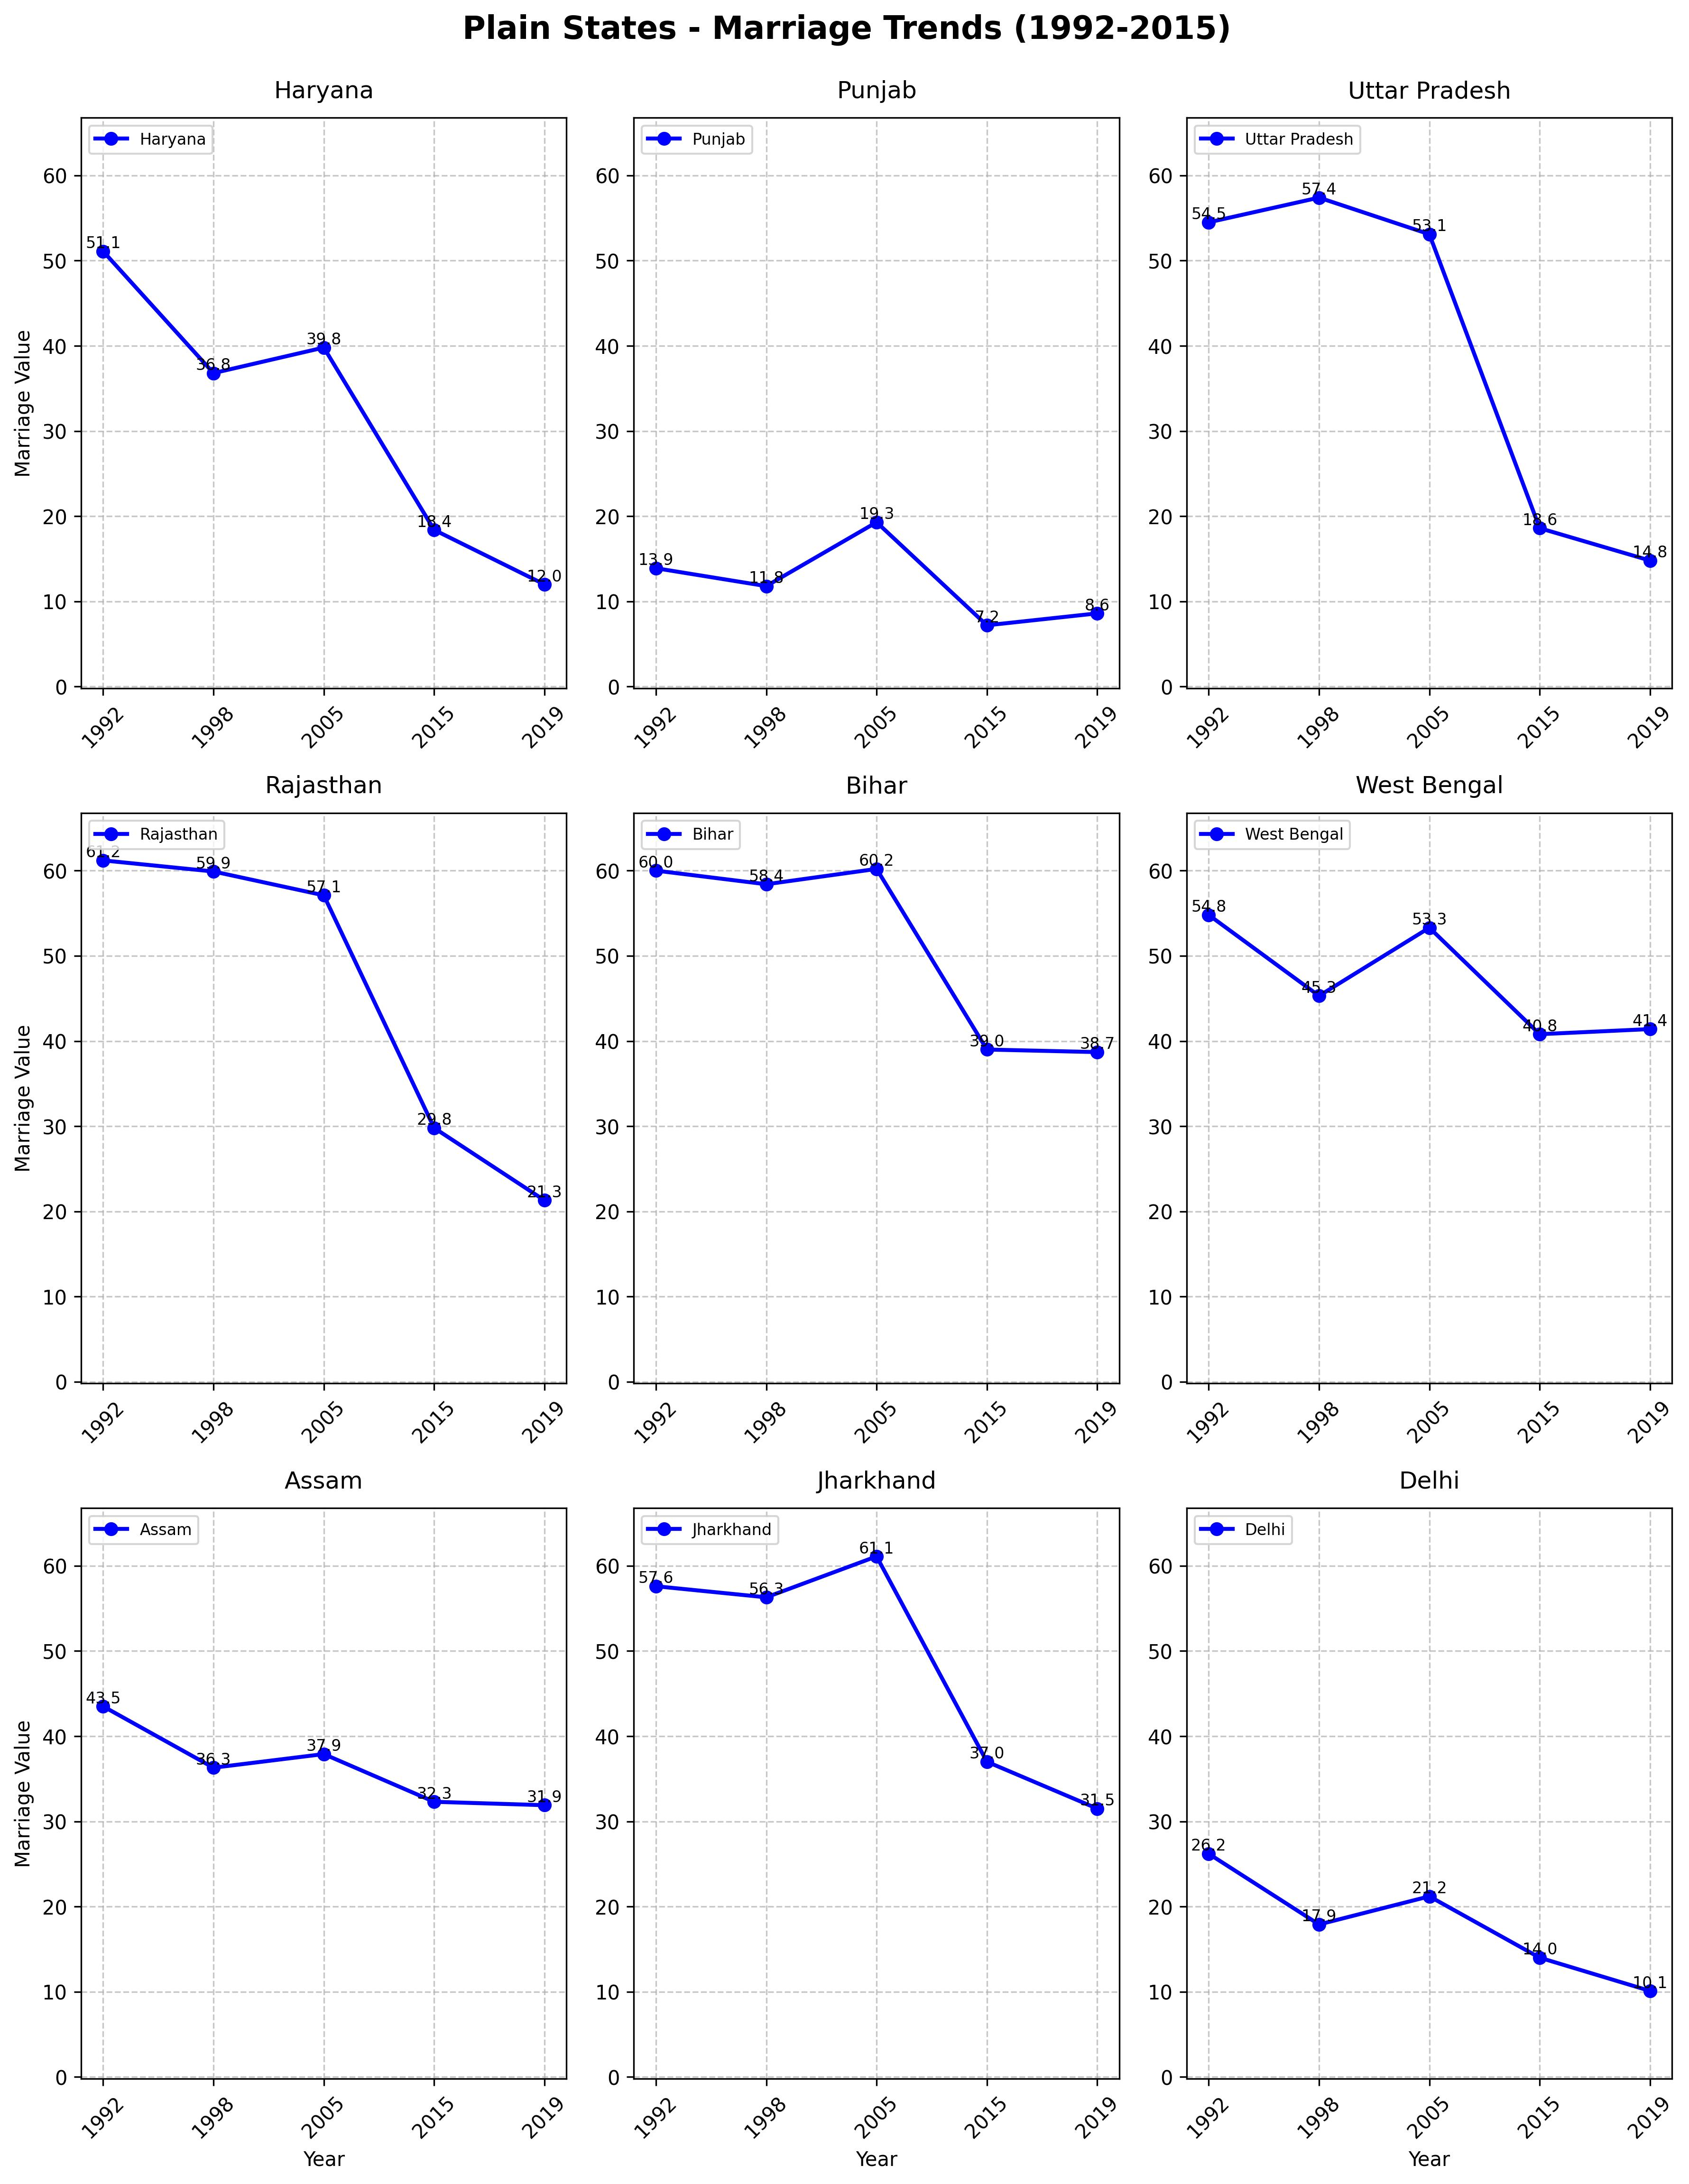
\includegraphics[width=0.9\textwidth]{figures/nfhs/plain_states_marriage_subplots.jpeg}
%     \caption{Child Marriage age in Plain States}
%     \label{fig:nfhs_plain_marriage}
% \end{figure}


% \begin{figure}[H]
%     \centering
%     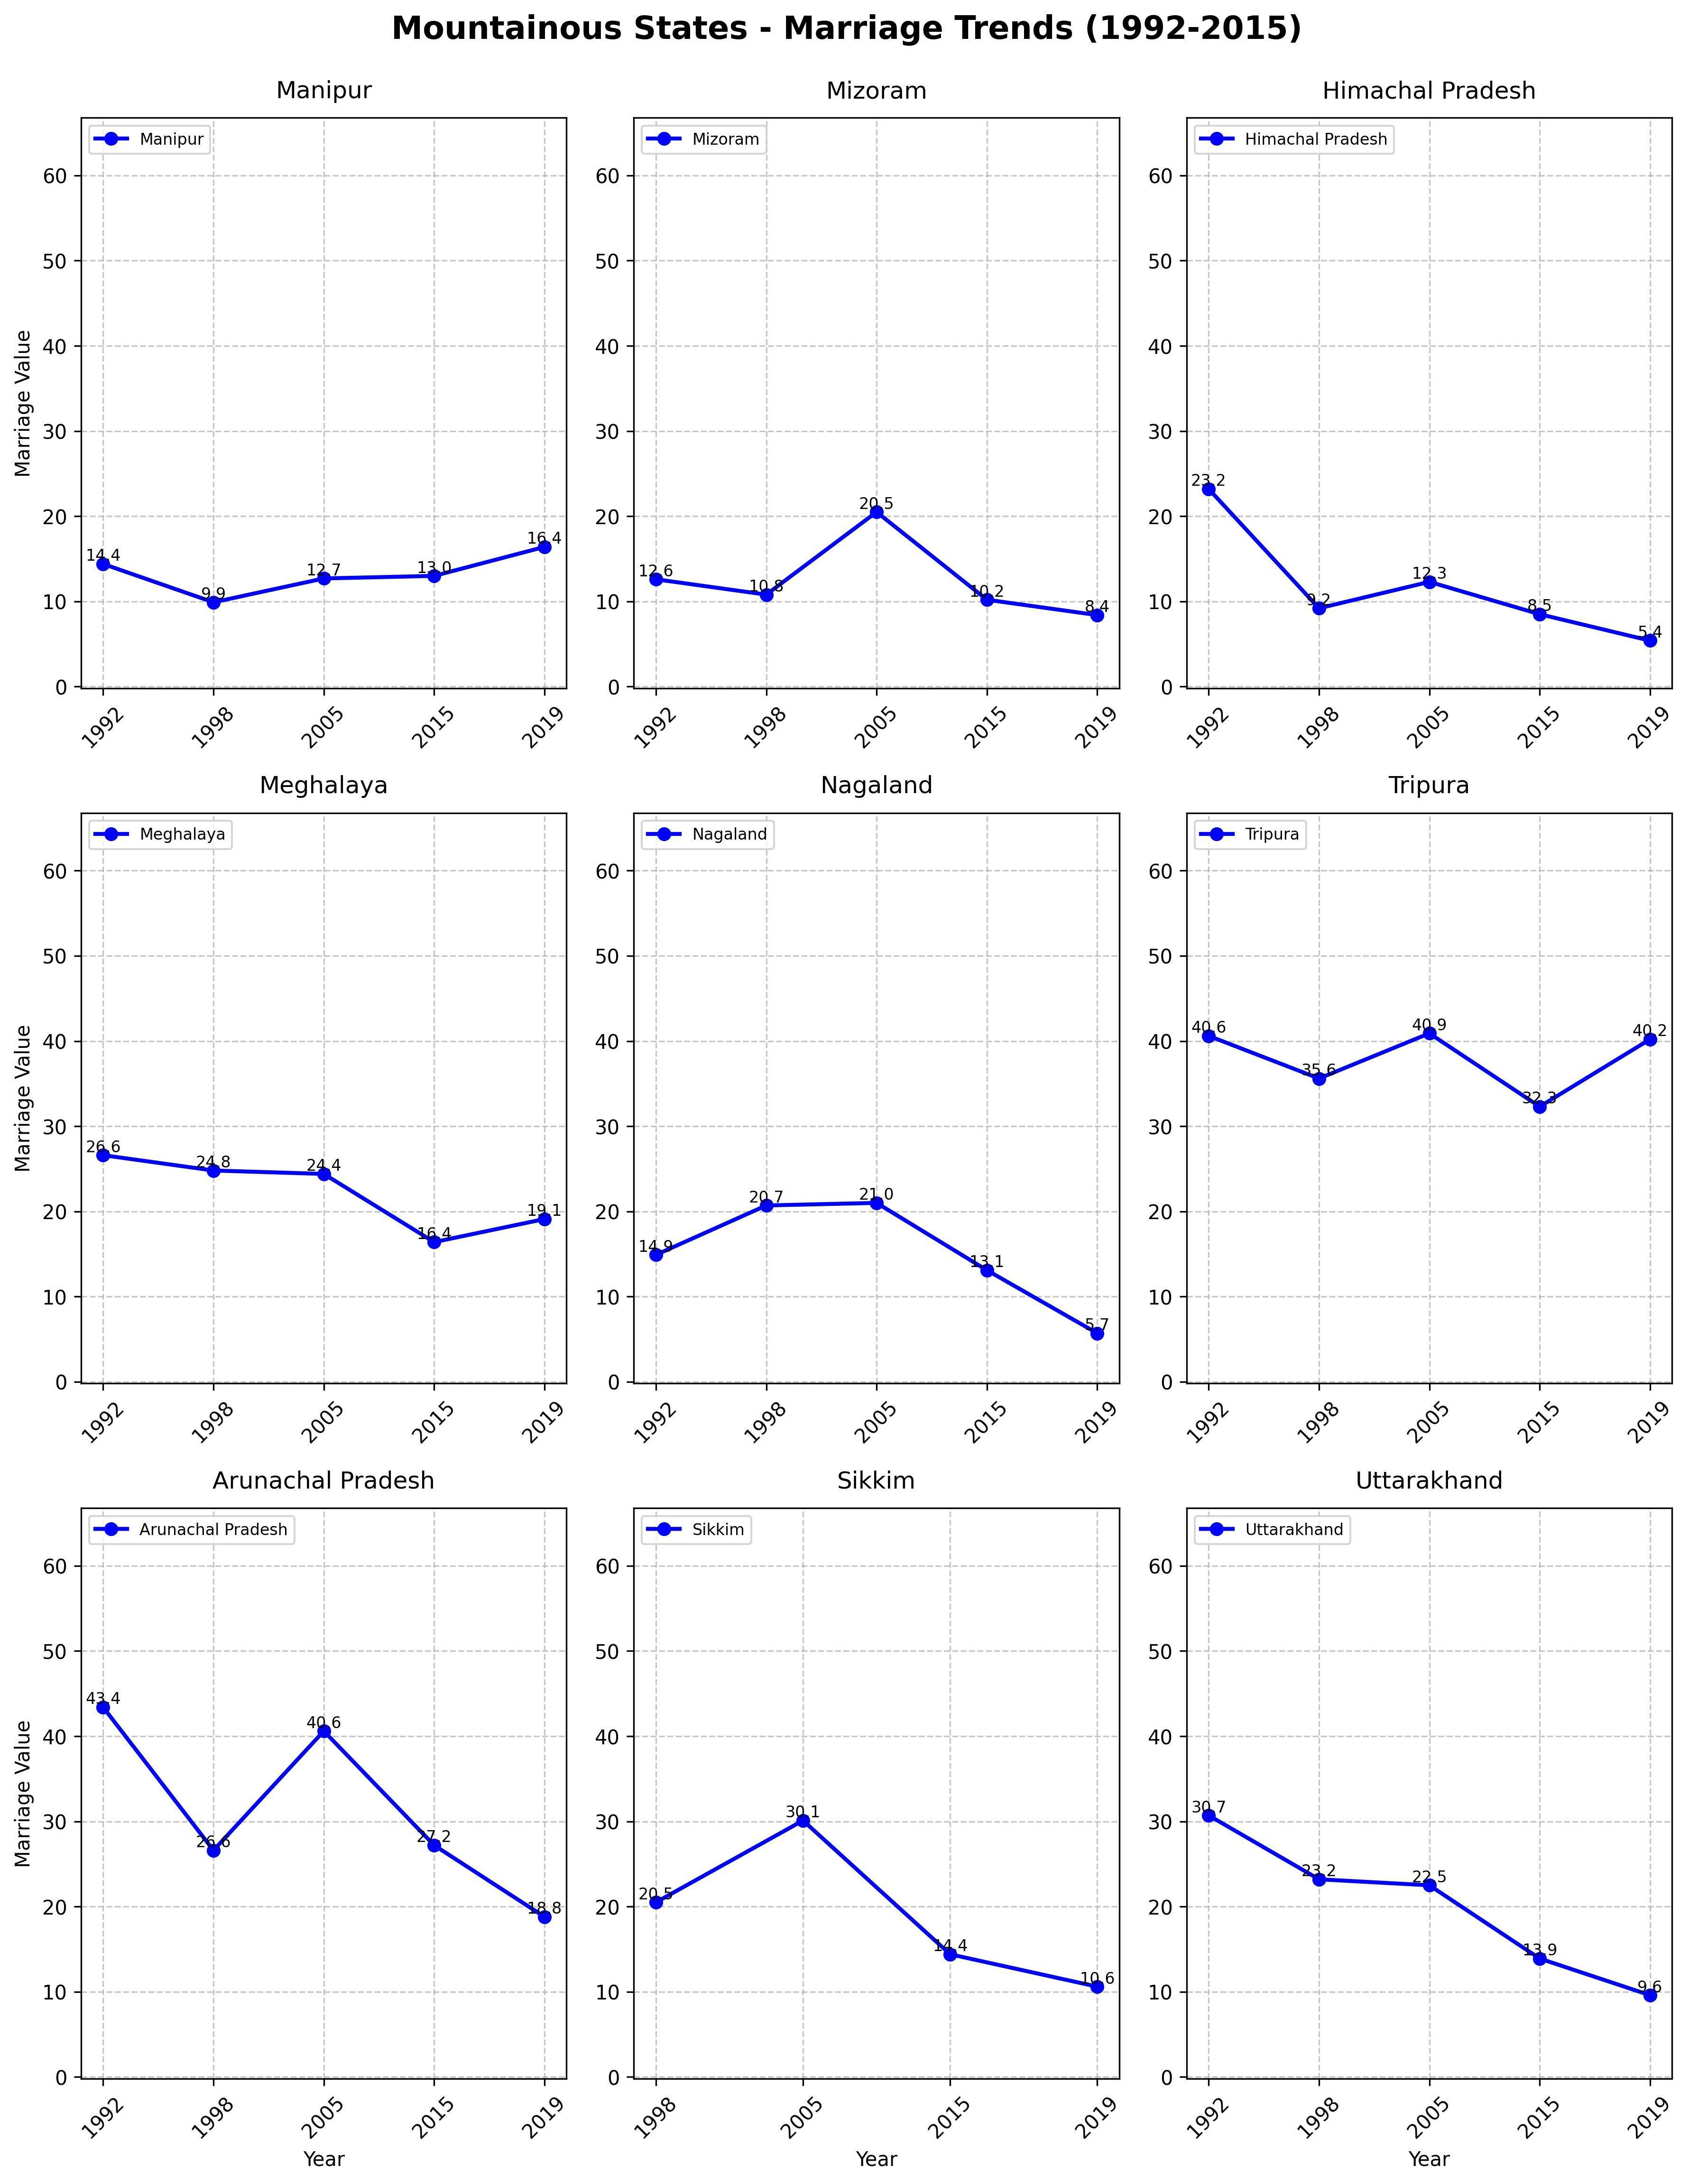
\includegraphics[width=0.9\textwidth]{figures/nfhs/mountainous_states_marriage_subplots.jpeg}
%     \caption{Child Marriage age in Mountain States}
%     \label{fig:nfhs_mountain_marriage}
% \end{figure}
The data in Table \ref{tab:child_marriage} suggests a clear trend of improvement across all states from 1992 to 2019 as the child marriage rates are decreasing, indicating progress in almost all the states. Himachal Pradesh, Mizoram, Manipur, Nagaland, Uttarakhand, and Sikkim all rank within the top ten. Arunachal Pradesh and tripura are the only two mountain states present in the bottom eight. Himachal Pradesh has secured the first position due to a steady and substantial decline in values over the years. Mizoram follows closely, showing consistently low values and strong improvement. In contrast, plain states display mixed performance. While Punjab and Delhi rank relatively high, states like Bihar, Rajasthan, and Jharkhand remain at the bottom despite showing progress. Overall, mountainous states tend to perform better overall as they dominate the top ranks.

\subsubsection{Literacy}
In Table \ref{tab:combined_literacy_states_diff} we can see that from 1991 to 2016, every state experienced a notable rise in literacy. The table \ref{tab:combined_literacy_states_diff} is ranked by the female literacy. Mizoram showed consistently high literacy at 82.26\% in 1991 and reaching 89.4\% in 2016, closely followed by Delhi, which showed a steep climb from about 62\% to nearly 94\%. Many mountainous or northeastern states appear near the top: Nagaland and Tripura share third place with values around 80\%, Himachal Pradesh and Uttarakhand show robust improvements (both surpassing 80\% by 2016), and Sikkim moves from 46.76\% to 76.43\%. Plain states have showed consistenly low literacy as visible that all the bottom four states are plain states and no state apart from Punjab came in the top five. Nagaland interestingly presents a nearly negligible gap (with an average difference of -0.49), implying that the female literacy rates are almost on par with the male rates. The calculated differences (Avg. Male - Avg. Female) are predominantly positive, confirming that male literacy rates tend to be higher than female rates in most regions.  This, along with  the fact that differential between average female and male literacy is very high in plain sates. Haryana, Uttar Pradesh, Jharkhand, Rajasthan and Bihar have a differential $\geq$ 20\%. Uttarakhand and Manipur are the on the highest side of differential in case of Mountains. Seven of the top ten states are mountain states with only Arunachal Pradesh in the bottom eight.  There has been a greater percentage increase in the proportion of females gaining literacy in all states due to the consolidated efforts of the government. Overall, mountain states performed better than plain states in this parameter.
\begin{table}[h]
    \centering
    % Added an extra column for the difference
    \begin{tabular}{lccccccccccc}
        \toprule
        \textbf{State} & \multicolumn{5}{c}{\textbf{Female Literacy (\%)}} & \multicolumn{5}{c}{\textbf{Male Literacy (\%)}} & \textbf{Diff.} \\
        \cmidrule(lr){2-6} \cmidrule(lr){7-11}
        & 1991 & 2001 & 2011 & 2017 & Avg. & 1991 & 2001 & 2011 & 2017 & Avg. & (M-F) \\
        \midrule
        Mizoram          & 82.26 & 86.75 & 89.27 & 89.40 & 86.92 & 93.35 & 95.00 & 93.35 & 93.72 & 93.86 & 6.94 \\
        % Delhi           & 61.99 & 74.71 & 80.76 & 93.70 & 77.79 & - & - & - & - & - & - \\  
        Nagaland        & 61.92 & 76.11 & 76.11 & 80.11 & 73.56 & 61.65 & 66.59 & 82.75 & 83.29 & 73.07 & -0.49 \\
        Tripura         & 49.56 & 73.19 & 82.73 & 83.15 & 72.16 & 81.47 & 91.53 & 92.53 & 92.18 & 89.43 & 17.27 \\
        Himachal Pradesh & 52.13 & 67.42 & 75.93 & 80.50 & 69.00 & 75.36 & 85.35 & 89.53 & 92.90 & 85.79 & 16.79 \\
        Punjab          & 50.41 & 63.55 & 70.73 & 78.50 & 65.80 & 65.66 & 75.23 & 80.44 & 88.50 & 77.46 & 11.66 \\
        Uttarakhand     & 52.28 & 60.26 & 70.01 & 80.70 & 65.81 & 86.60 & 92.00 & 87.40 & 94.30 & 90.08 & 24.27 \\
        Sikkim          & 46.76 & 60.40 & 75.61 & 76.43 & 64.80 & 76.73 & 86.55 & 86.55 & 87.29 & 84.28 & 19.48 \\
        West Bengal     & 48.64 & 60.22 & 70.54 & 76.10 & 63.88 & 73.00 & 77.58 & 81.69 & 84.80 & 79.77 & 15.89 \\
        Manipur         & 47.60 & 60.53 & 70.26 & 73.17 & 62.39 & 86.49 & 90.00 & 83.58 & 86.49 & 86.14 & 23.75 \\
        Meghalaya       & 44.85 & 59.61 & 72.89 & 73.78 & 62.78 & 60.65 & 65.43 & 75.95 & 77.17 & 69.80 & 7.02 \\
        Assam           & 43.03 & 56.03 & 66.27 & 81.20 & 61.63 & 61.87 & 71.28 & 77.85 & 90.10 & 75.28 & 13.65 \\
        Haryana         & 40.48 & 56.31 & 65.94 & 71.30 & 58.51 & 69.10 & 84.06 & 84.06 & 88.00 & 81.31 & 22.80 \\
        Arunachal Pradesh & 29.69 & 44.24 & 57.70 & 59.50 & 47.28 & 51.50 & 64.07 & 72.55 & 73.40 & 65.38 & 18.10 \\
        Uttar Pradesh   & 25.31 & 42.22 & 57.18 & 63.40 & 47.03 & 55.73 & 68.82 & 77.28 & 81.80 & 70.41 & 23.38 \\
        Jharkhand       & 25.50 & 39.38 & 55.42 & 64.70 & 46.75 & 67.94 & 78.45 & 76.84 & 83.00 & 76.56 & 29.81 \\
        Rajasthan       & 20.44 & 43.85 & 52.12 & 57.60 & 43.00 & 54.99 & 75.70 & 79.19 & 80.80 & 72.17 & 29.17 \\
        Bihar           & 22.89 & 33.12 & 51.50 & 60.50 & 42.00 & 59.68 & 60.32 & 71.20 & 79.70 & 67.73 & 25.73 \\
        \bottomrule
    \end{tabular}
    \caption{Male and Female Literacy Rates in Indian States (1991-2017) with Difference}
    \label{tab:combined_literacy_states_diff}
\end{table}

\subsubsection{Breast Milk}
\begin{table}[h!]
\centering
\begin{tabular}{lcccccc}
\toprule
\textbf{State} & \textbf{1992} & \textbf{1998} & \textbf{2005} & \textbf{2015} & \textbf{2019} & \textbf{Final Rank} \\
\midrule
Sikkim             & --   & 87.3  & 70.1  & 49.9  & 54.7  & 1  \\
Manipur           & 50   & 86.8  & 55.3  & 36.9  & 39.0  & 2  \\
Meghalaya         & 56.3 & 77.1  & 35.3  & 45.4  & 51.0  & 2  \\
West Bengal       & 53.6 & 46.3  & 58.7  & 36.6  & 50.7  & 4  \\
Mizoram           & 64.3 & 74.2  & 35.0  & 41.2  & 33.7  & 5  \\
Himachal Pradesh  & 39.9 & 61.3  & 69.2  & 24.5  & 31.1  & 6  \\
Tripura           & 65.0 & --    & 56.8  & 15.1  & 25.6  & 7  \\
Arunachal Pradesh & 35.8 & 60.2  & 33.8  & 33.3  & 40.0  & 8  \\
Nagaland          & 43.5 & 81.3  & 27.7  & 33.2  & 21.8  & 9  \\
Delhi             & 25.1 & 37.0  & 51.5  & 24.1  & 30.8  & 10 \\
Assam             & 39.2 & 58.5  & 32.7  & 27.8  & 23.4  & 11 \\
Punjab            & 37.3 & 38.7  & 39.9  & 15.6  & 26.7  & 12 \\
Uttarakhand       & --   & --    & 47.9  & 19.8  & 20.6  & 13 \\
Haryana           & 38.5 & 41.8  & 31.3  & 16.4  & 21.7  & 14 \\
Bihar             & 18.1 & 15.0  & 34.9  & 16.8  & 19.6  & 15 \\
Uttar Pradesh     & 19.4 & 17.3  & 36.1  & 9.8   & 15.2  & 16 \\
Jharkhand         & --   & --    & 28.5  & 13.8  & 21.2  & 17 \\
Rajasthan         & 9.4  & 17.5  & 20.8  & 8.5   & 16.3  & 18 \\
\bottomrule
\end{tabular}
\caption{States with Final Rank for Breast Milk}
\label{tab:breastmilk_rank}
\end{table}

The table \ref{tab:breastmilk_rank} illustrates the performance of various states in terms of how much breast milk and solid/mushy food is fed to children by women. Most states display  upward trends, indicating more maternal agency. Sikkim shows strong progress by 1998 as it ranks first. In contrast, states like Rajasthan and Uttar Pradesh, with modest or fluctuating values, fall toward the lower end of the ranking. Apart from Uttarakhand, all mountain states are present in top 10. Only West Bengal comes on rank 4 among all the mountain states. Overall, the mountain states clearly outperform the plain states in this case. Studies have shown that higher maternal self‐efficacy and positive ideational factors (such as accurate knowledge about the benefits of breastfeeding and confidence in one’s ability to nurse) are closely associated with improved breastfeeding practices. This indirectly measures the agency of a mother in her decision on health and care \citep{Hutchinson_2022}
\subsubsection{Contraceptive Data}

\begin{table}[h!]
\centering
\caption{Contraceptive Data}
\begin{tabular}{lcccccc}
\toprule
State & 1992 & 1998 & 2005 & 2015 & 2019 & Final\_Rank \\
\midrule
West Bengal & 57.4 & 66.6 & 71.2 & 70.9 & 74.4 & 1 \\
Himachal Pradesh & 58.4 & 67.7 & 72.6 & 56.8 & 74.2 & 2 \\
Delhi & 60.3 & 63.8 & 66.9 & 54.8 & 76.4 & 3 \\
Punjab & 58.7 & 66.7 & 63.3 & 75.8 & 66.6 & 4 \\
Tripura & 56.1 &  & 65.7 & 64.1 & 71.2 & 5 \\
Haryana & 49.7 & 62.4 & 63.4 & 63.7 & 73.1 & 6 \\
Uttarakhand &  &  & 59.3 & 53.4 & 70.8 & 7 \\
Rajasthan & 31.8 & 40.3 & 47.2 & 59.7 & 72.3 & 8 \\
Sikkim &  & 53.8 & 57.6 & 46.7 & 69.1 & 9 \\
Assam & 42.8 & 43.3 & 56.5 & 52.4 & 60.8 & 10 \\
Mizoram & 53.8 & 57.7 & 59.9 & 35.3 & 31.2 & 11 \\
Manipur & 34.9 & 38.7 & 48.7 & 23.6 & 61.3 & 12 \\
Uttar Pradesh & 19.8 & 28.1 & 43.6 & 45.5 & 62.4 & 13 \\
Jharkhand &  &  & 35.7 & 40.3 & 61.7 & 14 \\
Arunachal Pradesh & 23.6 & 35.4 & 43.2 & 31.6 & 59.1 & 15 \\
Nagaland & 13 & 30.3 & 29.7 & 26.5 & 57.4 & 16 \\
Bihar & 23.1 & 24.5 & 34.1 & 24 & 55.8 & 17 \\
Meghalaya & 20.7 & 20.2 & 24.3 & 24.3 & 27.4 & 18 \\
\bottomrule
\end{tabular}
\label{tab:contraceptive_data}
\end{table}
Table \ref{tab:contraceptive_data} shows a constant increase in contraceptive usage in most states. The slight drop from NFHS-3 to NFHS-4 is questioned in the existing literature. Some researchers suggested it could be due to better survey rigor (reducing over-reporting), while others pointed to persistent unmet need and women’s limited say in contraceptive decisions \citep{kumar2022measuring}. The data for some states is missing due to different reasons but it is important to note that most mountain societies underperform in this parameter. Mizoram and Manipur, especially showed a great drop from NFHS-3 (2005) to NFHS-4 (2015) which effected there rankings greatly. Most plains, however show high rates of contraceptive use consistently without varied fluctuations even across NFHS-3 to NFHS-4. Plain states like West Bengal, Himachal, Delhi and Haryana have shown better results than the mountain states. A major reason for this in existing literature is  the accessibility to the modern contraceptive methods in the remote mountain regions leading to a lesser usage. 

\subsubsection{Final Rank}
 The table \ref{tab:consolidated_ranks} is made from the final rankings of the parameters described above and methodology used from section \ref{ranking_methodology}. For recap, each parameter is given the same weight in the ranking. A lower rank here indicates better performance. We can observe that the mountain states clearly outperform the plain states. In the bottom seven ranks, only one state is a mountain state. Apart from Punjab and Delhi, no plain state is a part of the top seven. This clearly shows that mountain states have better agency, freedom for women with lesser exploitation. The difference between plain and mountain states is noticed in various studies implicitly \citep{kishor2004women} but the reasons are varied. Better infrastructure, cultural reasons, more acceptance for women are cited to be the leading reasons. However, due to remoteness mountain regions often have modest infrastructure compared to their plain counterparts. The results here suggest that something more fundamental is at play. We will explore these reasons in the next chapter.
\begin{table}[h!]
\centering
\begin{tabular}{|l|c|}
\hline
\textbf{State} & \textbf{Final Rank} \\
\hline
Himachal Pradesh & 1 \\
Mizoram & 2 \\
Delhi & 3 \\
Punjab & 4 \\
Sikkim & 5 \\
Manipur & 6 \\
Tripura & 7 \\
West Bengal & 8 \\
Nagaland & 9 \\
Uttarakhand & 10 \\
Meghalaya & 11 \\
Haryana & 12 \\
Assam & 13 \\
Arunachal Pradesh & 14 \\
Uttar Pradesh & 15 \\
Rajasthan & 16 \\
Jharkhand & 17 \\
Bihar & 18 \\
\hline
\end{tabular}
\caption{Consolidated Final Ranks of States}
\label{tab:consolidated_ranks}
\end{table}
\section{Conclusion}
The analysis in the chapter reveals how mountain and plain states behave differently. The Indo Gangetic plains exhibit a consistent divergence from the two party system in both lok and assembly level elections. The mountain states on the other hand converge strongly in both, however the value is higher than the softer threshold in assembly elections. Regardless, the converging nature suggests that there is a strong difference between the geographies. To examine the social indicators, we analyze various aspects of women's lives across both mountain and plain states. Mountain states generally rank higher in indicators related to women's empowerment, including literacy, breastfeeding practices, and reduced rates of child marriage. However contraceptive use is limited due to the remoteness. These indicators indicate higher maternal agency, better decision making for women, better health etc. In the next chapter we will evaluate the \textit{possible} reasons for the differences due to geography.